\Chapter{AngularJS implementáció}

CRUD műveletek megvalósítása: (CREATE, READ, UPDATE, DELETE) – Létrehozás, Lekérés, Frissítés, Törlés
Az web alkalmazásban ezeket a funkciókat a MMA harcosokon lehet végrehajtani.

A szerver által nyújtott REST API megvalósítása biztosítja a kód működőképességét.

A harcosokon végzett műveleteket a fighters.js nevű fájl tartalmazza.

Ahhoz, hogy minden megfelelően működjön létre kell hozni egy modult az alkalmazásban:

\begin{cpp}
var app = angular.module('app');
\end{cpp}

Ezután egy hozzátartozó kontrollert:

\begin{cpp}
app.controller('FightersController', ['$scope', '$http', '$location', 
'$stateParams',  '$state', function($scope, $http, $location, 
$stateParams, $state){
}]);
\end{cpp}

Ebbe a kontrollerbe tehetjük be a különböző funkciókat: A harcosok szerverről való lekérése:

\begin{cpp}
$scope.getFighters = function(){
$http({
	method: 'GET',
	url: '/api/fighters'
	}).then(function successCallback(response) {
	$scope.fighters = response.data;
	}, function errorCallback(response) {
});}
\end{cpp}

Ehhez egy GET kérést szükséges elküldeni a szervernek, ami visszaküldi egy response objektumban ez esetben a fighters objektumot, ami a harcosok adatait tartalmazza.

A /api/fighters URL-en lévő adatokat adja vissza, amik JSON formátumban vannak eltárolva.

A következő példakód egy harcos hozzáadását mutatja be, ehhez egy POST HTTP kérés elküldésére van szükségünk:

\begin{cpp}
$scope.addFighter = function(){
		console.log($scope.fighter);
		$http({
			method: 'POST',
			url: '/api/fighters/',
			data: $scope.fighter
		}).then(function successCallback(response) {
			$state.go("fighters");
		}, function errorCallback(response) {
  		});
	}
\end{cpp}

Miután a szerver sikeresen teljesítette a kérést, a \texttt{\$state.go("fighters");} kódsor
visszairányítja a felhasználót a ’fighters’ nevű route-ra, ami a /fighters oldallal egyezik meg.

Egy harcos adatainak frissítéséhez már szükség van a frissíteni kívánt harcos szerveren tárolt id mezőjére.

\begin{cpp}
$scope.updateFighter = function(){
		var id = $stateParams.id;
		$http({
			method: 'PUT',
			url: '/api/fighters/' +id,
			data: $scope.fighter
		}).then(function successCallback(response) {
			$state.go("fighters");
		}, function errorCallback(response) {
  		});
	} 
\end{cpp}

Ezt egy változó létrehozásával tehetjük meg, amiben letároljuk az id-t a 
\texttt{\$stateParams} segítségével, ami az URL-ből olvassa ki az id-t. Sikeres végrehajtás után a szerver ismét visszairányít a ’fighters’ nevű route-ra, tehát a /fighters oldalra, hogy lássuk a végrehajtott változtatásokat.

Egy harcos törléséhez szintén szükségünk van az id-jére, amit a megfelelő HTML oldalon lévő törlés gombnál adunk meg neki, ami a megfelelő harcos id-jével hívja meg a removeFighter nevű függvényt.

\begin{cpp}
$scope.removeFighter = function(id){
		$http({
			method: 'DELETE',
			url: '/api/fighters/' +id,
			data: $scope.fighter
		}).then(function successCallback(response) {
			$state.go("fighters");
		}, function errorCallback(response) {
  		});
	}
\end{cpp}

A következő funkció a harcosok táblázatának betűsorozatra való leszűkítése. Ekkor, ha a felhasználó egy kereső mezőbe begépel egy betűt, vagy betűsorozatot, amit az egyik, vagy több harcos neve tartalmaz, akkor a táblázat, ami megjeleníti a harcosokat dinamikusan szűkül le, és mutatja azt, vagy azokat a harcosokat, akinek, vagy akiknek a nevére illik a keresőmező tartalma.

\begin{cpp}
<div id="search">
  <input type="text" ng-model="search.name" 
  placeholder="Search fighters..."/>
</div>
\end{cpp}

Az kereső mezőn kívül szükség van egy filterre is, amit a \texttt{<table>} \texttt{<tbody>} részének első sorába írhatunk be: ez jeleníti meg az egyes harcosok nevét, becenevét, és egy View Details feliratú linket, amire kattintva megtekinthetők az adott harcos adatai.

\begin{cpp}
<tbody>
	<tr ng-repeat="fighter in fighters | filter:search">
		<td>{{ fighter.name }}</td>
        <td>{{ fighter.nickname }}</td>
	</tr>
</tbody>
\end{cpp}

\Section{Form validáció}

A form validáció többféle módon valósítható meg.
Az egyik megvalósítási lehetőség a \texttt{\$valid} és \texttt{\$invalid} state-ekkel (állapot):

\begin{cpp}
<form name="fighterForm" ng-submit="addFighter(fighterForm.$valid)" 
novalidate>
\end{cpp}

A novalidate kulcsszó ahhoz szükséges, hogy kikapcsoljuk a HTML5 alapvető validációs funkcióját.

\begin{cpp}
<button type="submit" ng-disabled="fighterForm.$invalid" 
		class="btn btn-default">Submit</button>
\end{cpp}

Ha a form még nem érvényes (valid) akkor a Submit (elküldés) gombra való kattintás letiltásra kerül, így a felhasználó nem tudja elküldeni a form-ot.

Szöveg mezők validációját a következőképpen valósítottam meg:

\begin{cpp}
<div class="form-group" ng-class="{ 'has-error' : 
fighterForm.name.$touched && !fighterForm.name.$dirty || 
fighterForm.name.$invalid && !fighterForm.name.$pristine }">
<label>Name*</label>
<input type="text" class="form-control" name="name" 
ng-model="fighter.name" placeholder="Name" ng-minlength="3" required/>
<p ng-show="fighterForm.name.$touched && !fighterForm.name.$dirty && 
!fighterForm.name.$error.minlength || fighterForm.name.$invalid && 
!fighterForm.name.$pristine && !fighterForm.name.$error.minlength" 
class="help-block">Name is required.</p>
<p ng-show="fighterForm.name.$error.minlength" class="help-block">
    Name is too short.</p>
</div>
\end{cpp}

Az alkalmazás akkor írja ki a validációs hibaüzenet, ha egyszerre teljesülnek az alábbi feltételek:
\begin{itemize}
\item az input mezőbe kattint a felhasználó, de nem ír a mezőbe semmit 
\item vagy ha a mező értéke nem érvényes, pedig már írt bele
\end{itemize}

A hibaüzenet a mezőből való kikattintás után jelenik meg. A név mező kötelező hibaüzenet (Name is required.) csak abban az esetben jelenik meg, ha a mező üres, tehát a minimum karakterszám nem teljesülése még nem lehet hiba.

Amint a felhasználó beleír valamit a mezőbe, a „Name is required” hibaüzenet eltűnik és a Név túl rövid (Name is too short.) hibaüzenet jelenik meg egészen addig, amíg a név mező karaktereinek száma el nem éri a 3-at.

A has-error ng-class (AngularJS osztály) hiba esetén a hibaüzenetnek piros színnel és a beviteli mezőnek piros szegéllyel való megjelenítéséért felelős.

A szám mezőknél a min és max direktívákat használtam:

\begin{cpp}
<label>Height*</label>
<input type="number" class="form-control" name="height" 
ng-model="fighter.height" placeholder="Height" min="155" max="205" 
required/>
\end{cpp}

Az előző példához hasonlóan a „Height is required” hibaüzenet nem jelenik meg, csak üres mező esetében. Ezután, ha a beírt számérték nem 155 és 205 közé esik, akkor a 
„Height value must be between 155 and 205 cm.” hibaüzenet jelenik meg.

A record mezőnél az ng-pattern direktívával szűkítettem le a lehetséges megadható eseteket:

\begin{cpp}
<label>Record*</label>
<input type="text" class="form-control" name="record" 
ng-model="fighter.record" placeholder="Record" 
ng-pattern="/^[0-9]{1,2}-[0-99]{1,2}-[0-99]{1,2}$/" required/>
\end{cpp}

Ezzel elérhető, hogy csak akkor legyen érvényes a record mező értéke, ha az [0-999]-[0-999]-[0-999] formátumú. Ezt a mezőt is kötelező kitölteni így itt is csak akkor jelenik meg a „Record is required” hibaüzenet, ha még nem írt a felhasználó a mezőbe.

Ezután ha nem a fent említett formátumban írt a felhasználó a mezőbe, akkor a „The record must be in Wins-Draws-Losses form.” hibaüzenet jelenik meg, ami azt jelenti, hogy a rekord mezőt győzelem-döntetlen-vereség formában kell kitölteni, például: 30-2-3.

Az image\_url-hez hozzáadott
\begin{cpp}
ng-pattern="/^https?://.+$/"
\end{cpp}
direktívával pedig a harcos avatarjának URL link validációját készítettem el, ami ha a felhasználó nem http:// vagy https://-el kezdődő URL címet ad meg, akkor „Image URL must be valid.” hibaüzenetet kap.

\Section{Routing}

Az oldalak közötti routing az ui.router szervízzel van megoldva.
Ehhez az angular module-ba meg kell adnunk az ui.router-t, mint függőséget (dependency).

\begin{cpp}
angular
    .module('app', ['ui.router']);
\end{cpp}

Az alábbi kód /fighters oldal megjelenítését biztosítja, a FightersController biztosítja a funkciókat, a /fighters oldalra való navigációkor pedig az alkalmazás a fighters.html template-t tölti be.

\begin{cpp}
$stateProvider
.state('fighters', {
        url: '/fighters',
        controller: 'FightersController',
        templateUrl: 'app/views/fighters.html',
        controllerAs: 'vm' });
\end{cpp}

\Section{Projekt struktúra}

\begin{figure}[htb]
\centering
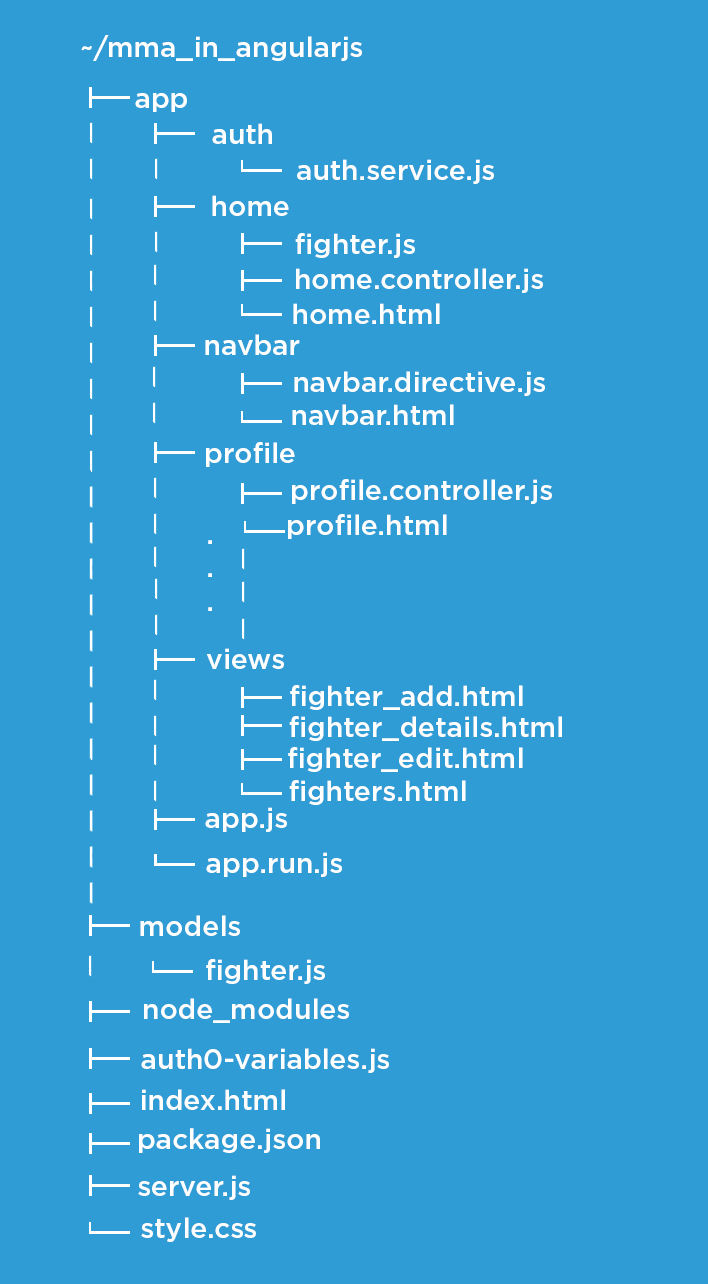
\includegraphics[scale=0.8]{kepek/mma_in_angularjs.jpeg}
\caption{Az AngularJS projekt struktúrája}
\label{fig:angularjs_structure}
\end{figure}
